\documentclass[a4paper]{article}
\usepackage[utf8]{inputenc}
\usepackage[english]{babel}
%\usepackage[sc]{mathpazo}
%\linespread{1.05}         % Palatino needs more leading (space between lines)
\usepackage[T1]{fontenc}
%\usepackage[pdftex]{color,graphicx}
%\usepackage{colortbl}
%\usepackage{pdfpages}
\usepackage{fancyhdr}
%\usepackage{amsmath} % math environment
%\usepackage{listings}
\usepackage{xcolor, colortbl}
\usepackage{graphicx}
\usepackage{pdfpages}
\usepackage{setspace} % text spacing options
\usepackage{textcomp} % text symbols
\usepackage{multicol}
\usepackage{calc}
\usepackage{rotating}

%temp
\usepackage{lipsum}

\pagestyle{fancy}

%Define commands
\newcommand{\systemname}{Jenkins Pre-tested Commits}
\newcommand{\groupname}{Team $\Delta$}
\newcommand{\groupmembers}{
	Andreas Frisch \{andreas.frisch@gmail.com\}, \\
	Esben Skaarup \{esben.skaarup@gmail.com\}, \\
	Alexander W. Uldall \{morpmex@gmail.com\} \\
	Ronni Elken Lindsgaard \{ronni.lindsgaard@gmail.com\}, \\
	~
}

%Define colors
\definecolor{Gray}{gray}{0.8}
\definecolor{DarkGray}{gray}{0.4}

\lhead{Project Course: Development Studio}
\chead{}
\rhead{\systemname}
\lfoot{}
\cfoot{\thepage}
\rfoot{}

%Start section numbering from 0
\setcounter{section}{-1}

\begin{document}
\begin{titlepage}
	% Title
	\begin{center}
		\vspace*{4cm}
		\rule{\linewidth}{0.5mm}\\[0.4cm]
		{\huge \bfseries \systemname}
		\rule{\linewidth}{0.5mm}
	\end{center}
	\begin{flushleft}
		{
			\Large Project Course: Development Studio \\[0.1cm]
			{\it Assignment 4 - sprint 3}
		}
	\end{flushleft}
	\vspace*{4cm}
	
	% Authors
	\begin{flushleft}
		{\Large \groupname :} \\[0.1cm]
		{\Large \groupmembers} \\[0.3cm]
		{\Large \today}
	\end{flushleft}
\end{titlepage}
\newpage
\onehalfspacing
\setcounter{tocdepth}{2}
%\tableofcontents
%newpage

\section{This hand-in}
This assignment is written as part of the course {\it Project Course: Development Studio} at DIKU.

This assignment concerns itself with our results from the third sprint.
Furthermore we will briefly discuss the lessons learned and how they affect our
upcoming sprint.

Our customer, Praqma, wants a plug-in for the continuous delivery facilitator
Jenkins, which allows Jenkins to rollback broken commits, thus maintaining an
unpolluted, pristine, company truth repository.

Our code and backlogs can be found at
\begin{quote}
	https://github.com/pcds2013-team-delta/pretest-commit-plugin
\end{quote}

\section{Sprint retrospective}
\label{sec:sprint_retrospective}
This section will consist of three different yet related subjects. Firstly we
will discuss our sprint goals for this sprint -- that is the customer-related
goals and should be seen in addition to the course-related goals specified by
the assignment description. Secondly we will discuss briefly how this sprint
turned out -- what worked and what did not. Lastly we will briefly discuss any
conflicts we encountered during this sprint with regard to group team-work and
communication.

\subsection{Sprint goals}
The purpose of this sprint was to get ready for the first community release.
While this might seem like a daunting task -- especially since none of us have
any experience in that regard -- it is important to understand that a community
release does not necessarily mean a finished product. Instead, what we need to
have is a product that is usable given any constraints we may need to make this
happen. The point is then to test what functionality real users require, what
workflows they need supported in a final version and lastly a larger scale general
test than we could design in the same time frame.

Thus the major tasks for this sprint is the redesign of the user interface, the
proper workings of the queue, the bootstrapping of the system, concurrency
guarantees and lastly a clean way of presenting errors to the users.

\subsection{Sprint experience}
\begin{figure}[!ht]
	\centering
	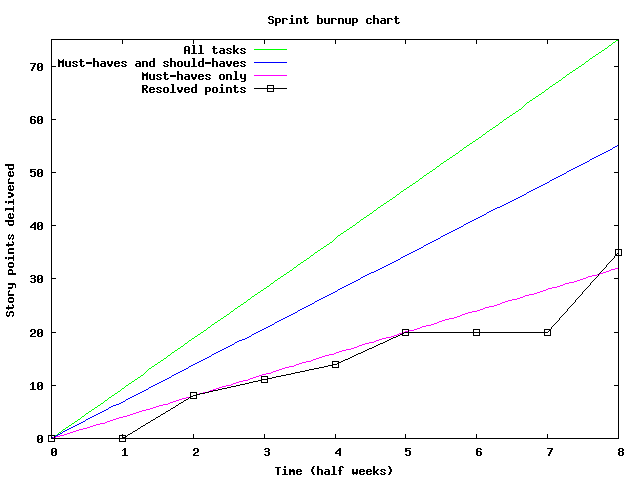
\includegraphics[width=\textwidth/2]{img/burndown.png}
	\caption{A burnup graph of our sprint 3.}
	\label{fig:burnup}
\end{figure}
Again for this sprint we experienced ``hard-to-close'' tasks due to both inter-task
dependencies and perfectionism on our part. This is apparent from the spikes in
our burnup chart (see figure \ref{fig:burnup}). Where properly defined tasks should give a
smooth curve following the desired line of efficiency, our tasks yield periods of
apparent inactivity followed by bursts of extreme efficiency.

We must become better at clearly defining our measurement of success regarding a
task, allowing us to mark it as complete. Further, we must accept when a task is
complete according to the task description, instead of continuing work due to
unforeseen errors that should be tasks on their own. This decision to stop a task
in a way that feels premature should, of course, be taken on a task to task
basis, as some emerging errors \textit{do} need immediate action.

Overall, however, we did get a lot of work done this sprint as well and while the
theoretical parts got down-prioritized more than we would have initially liked,
the important parts -- getting ready for a community release -- recieved a lot of
work.

\subsection{Group conflicts}
At the very beginning of the course, we put down some rules of conduct for the
group with special regard to intra-group communication. However, at that time
we merely wrote down some obvious truths, expecting all of us to share the same
type of humor and expecting all of us to be used to the general tone at DIKU --
especially regarding the friendly bashing of foreign operating systems, editors,
languages and every other digital choice.

Unfortunately this alignment was on paper only and during this sprint a member
of our group felt persecuted for his choice of operating system due to constant
quips. The rest of the group, having meant no harm, handled the situation badly
as we did not expect this tone to have seriously offended anybody.

Thus the situation escalated out of proportion, but after having talked the
situation over we are back on track -- working together as before. Having talked
things over, we are sure we can avoid such conflicts in the future, as we are
now more aware of possible subtle differences in our individual take on the
initial rules of conduct.

In the future -- beyond the scope of this project -- we might be able to construct
better rules of conduct, simply by having experienced how a loose approach to
defining those combined with a poorly defined
conflict handling strategy allows simple conflicts to escalate.

\section{Sprint learning goal}
\label{sec:learning_goals}
This section will consist of the three parts outlined in the assignment
description, namely an Architectural description of our system, documentation
of our entities and lastly the insights gained from having our code inspected
by another group.

\subsection{Architectural description}
\begin{figure}[!ht]
	\centering
	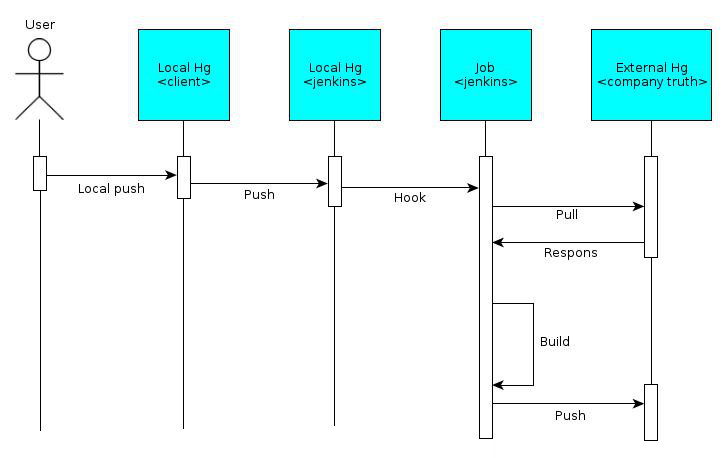
\includegraphics[width=8cm]{../graphs/sequence_diagram.jpg}
	\caption{Sequence diagram describing the general inter-system communication
	in the most common scenario. As seen there is no user interaction from the
	moment when the user pushes his updates.}
	\label{fig:dia_sequence}
\end{figure}
\begin{figure}[!ht]
	\centering
	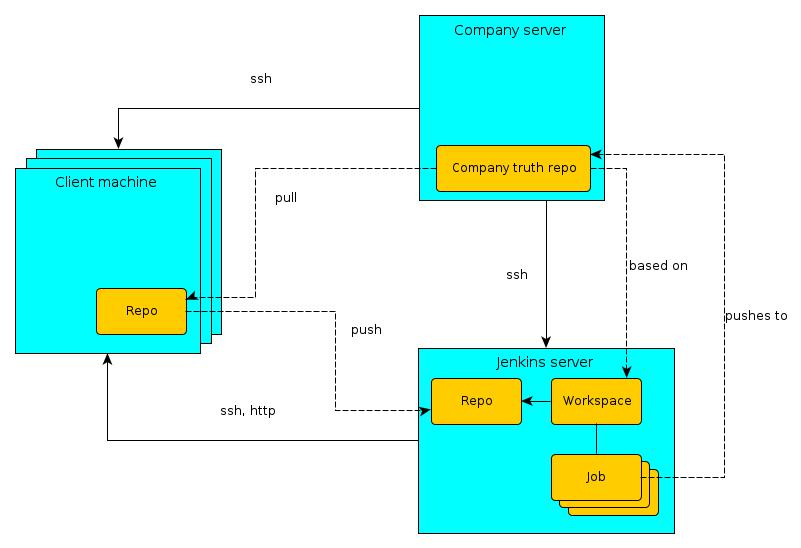
\includegraphics[width=8cm]{../graphs/architecture_01.jpg}
	\caption{Architectural diagram describing all major components, their
	internal relationships and the communication protocols they use. When no
	protocol is mentioned, this is determined by the desired SCM.}
	\label{fig:dia_architecture}
\end{figure}

Based on Christensen et al. 2011, this section will describe our current
system and the underlying architecture. This will not be a restatement of the
problem we are trying to solve; for that, please refer to the previous assignments.
Instead of using the three viewpoints presented in the article, however, we did
the following.

Figures \ref{fig:dia_sequence} and \ref{fig:dia_architecture} give an overview of
the various parts involved in the system as well as their connectors. These
diagrams yields a similar overview as the \texttt{Module} and
\texttt{Component \& Connector} viewpoints combined, but this rendition made more
sense when we tried to apply the theory to our own project. The \texttt{Allocation}
viewpoint is not as relevant for our product, as it is based on existing technology
and thus shares requirements with those. The parts of the \texttt{Allocation} viewpoint
not implicitly covered by host technologies are covered by the aforementioned diagrams.

Figure \ref{fig:dia_sequence} shows communication between different elements of
the system. These elements are individual entities either separated in code or
physically on different machines. While such a scenario diagram often features
specific function names as arrow labels, we decided against this to clearly
indicate how most operations between elements are part of the host technologies
and not something we have written. We also added the external user, as the figure
then also serves to illustrate the intended use of the system.

Figure \ref{fig:dia_architecture} shows the different physically separated modules,
their constituent parts and the protocols through which we handle inter-module
communication. Some of the protocols are undefined as the parts communicating
across this link are both internal parts of Jenkins, why we do not care about the
specific protocol, as Jenkins handles this for us. 

\subsection{Entity documentation}
As the entities of a system usually comprises models of physical objects or actors,
this notion has little relevance for our case. Unlike a web-shop having both
customers, items for sale, suppliers, wish lists and more to model as well as
users and suppliers as external actors, our product has no direct interaction from
users and no objects to model. Documenting our entities thus devolves into the
trivial task of doing nothing.

If we instead regard entities as separate pieces of code, our entities becomes our
job handler before and after a build as well as our queue. Those are all
documented through javadocs style comments, why it seems silly to repeat that information
here.

\subsection{Code inspection}
\label{sec:inspection}
\paragraph{Giving} feedback based on code inspection learned us very little. The
group we inspected had nicely separated pieces of code, making it easy to get an
idea of what was going on in their system. Beyond the few bits of unfinished code
and various disagreements on style and naming conventions, the only bit that
really stuck out was a security issue, where passwords were sent around in
cleartext. While we could learn a bit from the clean seperation of classes, our
project is a plug-in which imposes some restrictions in this regard.

\paragraph{Receiving} feedback yielded but a few potential structural changes. Most
of the feedback we got revolved around coding style and convention, perhaps
partly due to the fact that our code is highly integrated with Jenkins, making
it hard to cleanly separate functionalities. However, there were some excellent
comments still, especially regarding our \texttt{PretestCommitPreCheckout.java},
\texttt{PretestCommitPostCheckout.java} and \texttt{HgUtils.java}, where a
clearer separation of concerns regarding SCM functionality would increase both
readability and maintainability.

Secondly the inspectors mentioned a lack of JavaDocs here and there, which of
course needs ammending.

Lastly, due to an error on our part, the \texttt{CommitQueue.java} was unused in
the code we handed out for expection. An error that had been corrected before
the inspection meeting.

\subsubsection{List of inspected files}
Table \ref{tab:inspection} lists the files inspected and the important anomalies
found for each given file. Only the critical anomalies are recorded here. For a
brief discussions on the lessons learned from the review, see section
\ref{sec:inspection}.

\begin{table}[!ht]
	\centering
	\begin{tabular}{| p{6cm} | p{5cm} |}
			\hline
			\textbf{File}&\textbf{Anomalies} \\
			\hline
			<General> & JavaDocs are missing or incomplete. \\
			\hline
			\texttt{CommitQueue.java} &
				The queue is currently unused and performs no task.\\
			\hline
			\texttt{HgUtils.java} &
				Refactor to increase seperation of layers. Create a better API
				for calling the built-in SCMs.\\
			\hline
			\texttt{PretestCommitPreCheckout.java} &
				As this file uses \texttt{HgUtils.java}, see that comment. \\
			\hline
			\texttt{PretestCommitPostCheckout.java} &
				As this file uses \texttt{HgUtils.java}, see that comment. \\
			\hline
			\texttt{PretestUtils.java} & \\
			\hline
		\end{tabular}
		\caption{Inspection results for each file sent to inspection. Anomalies based
		on personal preferences -- such as indentation, commentation style and in some
		cases naming conventions -- not included.}
		\label{tab:inspection}
\end{table}
\end{document}
